
%(BEGIN_QUESTION)
% Copyright 2009, Tony R. Kuphaldt, released under the Creative Commons Attribution License (v 1.0)
% This means you may do almost anything with this work of mine, so long as you give me proper credit

Calculate the echo times for both the total level (air/oil interface) and oil/water interface in this radar level measurement application:

$$\includegraphics[width=15.5cm]{i04218x01.eps}$$

Also, calculate the power reflection factors for both interfaces (air/oil and oil/water).

\vfil 

\underbar{file i04218}
\eject
%(END_QUESTION)





%(BEGIN_ANSWER)

This is a graded question -- no answers or hints given!

%(END_ANSWER)





%(BEGIN_NOTES)

$$x = vt$$

Remember that the distances we are dealing with here for echoes are {\it round-trip}, not {\it one-way}.  Therefore, the 2 meter surface ullage is actually a 4 meter round-trip distance for the echo:

\vskip 10pt

$$t_1 = {4 \hbox{ m} \over 3 \times 10^8 \hbox{ m/s}} = 13.33 \hbox{ ns}$$

\vskip 10pt

The round-trip time for the interface echo is a bit more complicated to calculate because there are two different speeds of light to consider: the speed of light through the air, and the speed of light through the oil.  Since the oil has a relative permittivity of 5, the speed of light through that medium is only 1.34 $\times$ 10$^{8}$ m/s rather than 3 $\times$ 10$^{8}$ m/s.  We may calculate the round-trip time through the oil and then add that time to the time of the first echo (the round-trip time through the air) to arrive at the total interface echo time:

\vskip 10pt

$$t_2 = {7.2 \hbox{ m} \over 1.34 \times 10^8 \hbox{ m/s}} + t_1 = 67.00 \hbox{ ns}$$

\vskip 30pt

As for power reflection factors, this is a function of the difference between media permittivities:

\vskip 10pt

$$R = {\left({\sqrt{\epsilon_{r2}} - \sqrt{\epsilon_{r1}}}\right)^2 \over \left(\sqrt{\epsilon_{r2}} + \sqrt{\epsilon_{r1}}\right)^2}$$

\vskip 10pt

Calculating the reflection factor for the air-oil interface:

$$R_{air-oil} = {\left({\sqrt{5} - \sqrt{1}}\right)^2 \over \left(\sqrt{5} + \sqrt{1}\right)^2} = 14.59\%$$

\vskip 10pt

Calculating the reflection factor for the oil-water interface:

$$R_{oil-water} = {\left({\sqrt{80} - \sqrt{5}}\right)^2 \over \left(\sqrt{80} + \sqrt{5}\right)^2} = 36.00\%$$

%INDEX% Measurement, level: radar

%(END_NOTES)


